\documentclass[11pt,a4paper]{article}

% ============================================================================
% PACKAGES
% ============================================================================

% Encoding and fonts
\usepackage[utf8]{inputenc}
\usepackage[T1]{fontenc}
\usepackage{lmodern}

% Page layout
\usepackage[margin=2.5cm]{geometry}
\usepackage{parskip}

% Graphics and colors
\usepackage{graphicx}
\usepackage{xcolor}
\usepackage{tikz}
\usetikzlibrary{shapes.geometric, arrows.meta, positioning, fit, backgrounds}

% Tables
\usepackage{booktabs}
\usepackage{longtable}
\usepackage{array}
\usepackage{multirow}

% Code listings
\usepackage{listings}
\usepackage{fancyvrb}

% Hyperlinks
\usepackage{hyperref}
\hypersetup{
    colorlinks=true,
    linkcolor=blue!70!black,
    urlcolor=blue!70!black,
    citecolor=blue!70!black
}

% Headers and footers
\usepackage{fancyhdr}
\pagestyle{fancy}
\fancyhf{}
\rhead{\textit{ctx Codebase Analysis}}
\lhead{\textit{\leftmark}}
\cfoot{\thepage}

% Math
\usepackage{amsmath}
\usepackage{amssymb}

% ============================================================================
% CUSTOM COLORS
% ============================================================================

\definecolor{rustcolor}{RGB}{183, 65, 14}
\definecolor{codegreen}{RGB}{40, 167, 69}
\definecolor{codegray}{RGB}{108, 117, 125}
\definecolor{codepurple}{RGB}{111, 66, 193}
\definecolor{backcolour}{RGB}{248, 249, 250}
\definecolor{criticalred}{RGB}{220, 53, 69}
\definecolor{warningorange}{RGB}{255, 193, 7}
\definecolor{successgreen}{RGB}{40, 167, 69}

% ============================================================================
% CODE LISTING STYLES
% ============================================================================

\lstdefinestyle{rustcode}{
    backgroundcolor=\color{backcolour},
    commentstyle=\color{codegray}\itshape,
    keywordstyle=\color{rustcolor}\bfseries,
    numberstyle=\tiny\color{codegray},
    stringstyle=\color{codegreen},
    basicstyle=\ttfamily\small,
    breakatwhitespace=false,
    breaklines=true,
    captionpos=b,
    keepspaces=true,
    numbers=left,
    numbersep=5pt,
    showspaces=false,
    showstringspaces=false,
    showtabs=false,
    tabsize=4,
    frame=single,
    rulecolor=\color{codegray!30},
    language=C,
    morekeywords={fn, let, mut, pub, struct, enum, impl, trait, use, mod, self, Self, async, await, where, dyn, Box, Vec, String, Option, Result, Ok, Err, Some, None}
}

\lstdefinestyle{sqlcode}{
    backgroundcolor=\color{backcolour},
    commentstyle=\color{codegray}\itshape,
    keywordstyle=\color{blue!70!black}\bfseries,
    numberstyle=\tiny\color{codegray},
    stringstyle=\color{codegreen},
    basicstyle=\ttfamily\small,
    breaklines=true,
    captionpos=b,
    keepspaces=true,
    numbers=left,
    numbersep=5pt,
    frame=single,
    rulecolor=\color{codegray!30},
    language=SQL
}

\lstdefinestyle{bashcode}{
    backgroundcolor=\color{backcolour},
    commentstyle=\color{codegray}\itshape,
    keywordstyle=\color{codepurple}\bfseries,
    basicstyle=\ttfamily\small,
    breaklines=true,
    captionpos=b,
    frame=single,
    rulecolor=\color{codegray!30},
    language=bash
}

\lstset{style=rustcode}

% ============================================================================
% CUSTOM COMMANDS
% ============================================================================

\newcommand{\ctx}{\texttt{ctx}}
\newcommand{\code}[1]{\texttt{#1}}
\newcommand{\file}[1]{\texttt{\color{codepurple}#1}}
\newcommand{\func}[1]{\texttt{\color{rustcolor}#1}}
\newcommand{\critical}[1]{\textcolor{criticalred}{\textbf{#1}}}
\newcommand{\warning}[1]{\textcolor{warningorange}{\textbf{#1}}}
\newcommand{\success}[1]{\textcolor{successgreen}{\textbf{#1}}}

% ============================================================================
% DOCUMENT INFO
% ============================================================================

\title{%
    \vspace{-1cm}
    \Huge\textbf{ctx Codebase Analysis}\\[0.5cm]
    \Large A Comprehensive Technical Review of the\\
    Context Generation and Code Intelligence CLI Tool
}

\author{%
    Generated by Automated Code Analysis\\[0.2cm]
    \small Using ctx code intelligence features
}

\date{\today}

% ============================================================================
% DOCUMENT BEGIN
% ============================================================================

\begin{document}

\maketitle

\begin{abstract}
This document provides a comprehensive analysis of the \ctx{} codebase, a Rust-based command-line tool for generating AI-ready context from codebases and providing code intelligence features including indexing, search, call graphs, and impact analysis. The analysis covers architecture, module responsibilities, code quality metrics, dependency relationships, and recommendations for improvement. The codebase consists of \textbf{548 symbols} across \textbf{20 source files} with \textbf{2664 edges} representing function calls and relationships.
\end{abstract}

\tableofcontents
\newpage

% ============================================================================
% INCLUDE SECTIONS
% ============================================================================

% ============================================================================
% EXECUTIVE SUMMARY
% ============================================================================

\section{Executive Summary}
\label{sec:executive-summary}

\ctx{} is a well-architected Rust command-line tool providing two main capabilities:

\begin{enumerate}
    \item \textbf{Context Generation} --- Formats source code for consumption by Large Language Models (LLMs), with intelligent filtering, multiple output formats, and streaming support.
    
    \item \textbf{Code Intelligence} --- Provides comprehensive code analysis including indexing, full-text search, semantic search with embeddings, call graph generation, and impact analysis.
\end{enumerate}

\subsection{Key Metrics}

\begin{table}[h]
\centering
\begin{tabular}{lr}
\toprule
\textbf{Metric} & \textbf{Value} \\
\midrule
Total Source Files & 20 \\
Total Symbols & 548 \\
Functions & 446 \\
Structs & 35 \\
Enums & 11 \\
Traits & 3 \\
Total Edges (Relationships) & 2,664 \\
\bottomrule
\end{tabular}
\caption{Codebase statistics overview}
\label{tab:overview-stats}
\end{table}

\subsection{Technology Stack}

The tool leverages several key technologies:

\begin{itemize}
    \item \textbf{Rust} --- Primary implementation language, providing memory safety and performance
    \item \textbf{Tree-sitter} --- Incremental parsing library for accurate AST extraction across multiple languages
    \item \textbf{SQLite} --- Persistent storage for symbols, edges, and compressed source code
    \item \textbf{DuckDB} --- In-memory analytical database for recursive graph queries
    \item \textbf{FTS5} --- Full-text search extension for SQLite
    \item \textbf{fastembed} --- Local embedding generation using all-MiniLM-L6-v2
    \item \textbf{clap} --- Command-line argument parsing
\end{itemize}

\subsection{Supported Languages}

\begin{table}[h]
\centering
\begin{tabular}{llll}
\toprule
\textbf{Language} & \textbf{Extensions} & \textbf{Parser} & \textbf{Status} \\
\midrule
Rust & \code{.rs} & tree-sitter-rust & Full \\
TypeScript & \code{.ts}, \code{.tsx} & tree-sitter-typescript & Full \\
JavaScript & \code{.js}, \code{.jsx}, \code{.mjs} & tree-sitter-javascript & Full \\
Python & \code{.py}, \code{.pyi} & tree-sitter-python & Full \\
Solidity & \code{.sol} & tree-sitter-solidity & Full \\
YAML & \code{.yaml}, \code{.yml} & N/A & File tracking only \\
\bottomrule
\end{tabular}
\caption{Supported programming languages}
\label{tab:languages}
\end{table}

\subsection{Quality Assessment Summary}

The codebase demonstrates solid Rust practices with clear module separation. However, analysis revealed areas requiring attention:

\begin{itemize}
    \item \warning{17 high-complexity functions} exceeding recommended fan-out thresholds
    \item \warning{13 duplicate code pairs} indicating potential for abstraction
    \item \success{Clean module separation} with well-defined responsibilities
    \item \success{Comprehensive test coverage} for core functionality
\end{itemize}

% ============================================================================
% ARCHITECTURE
% ============================================================================

\section{Architecture}
\label{sec:architecture}

\subsection{High-Level Overview}

The \ctx{} architecture follows a modular design with clear separation between context generation and code intelligence features. The system is organized into distinct layers, each with well-defined responsibilities.

\begin{figure}[h]
\centering
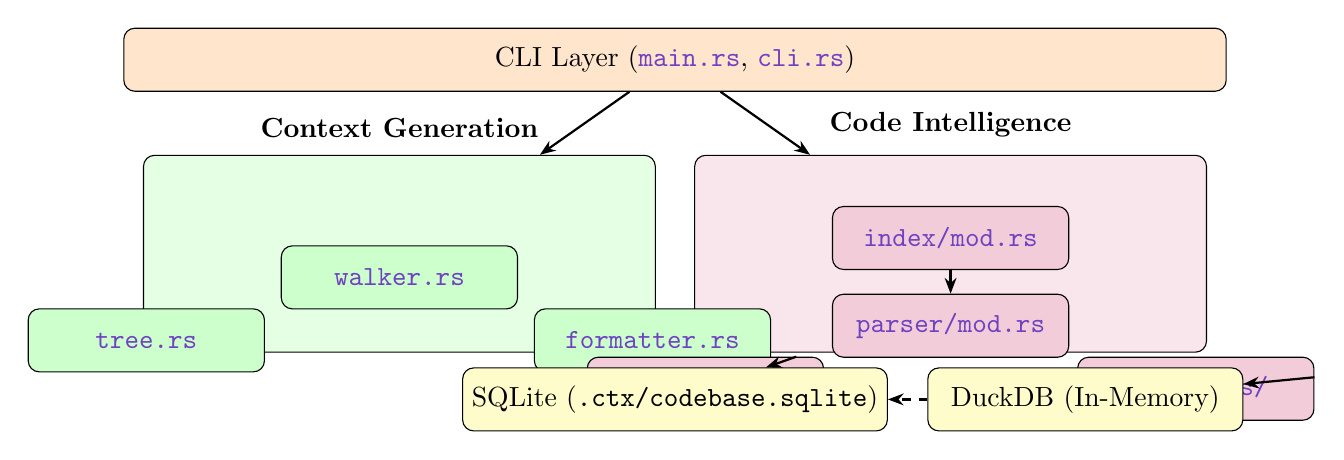
\begin{tikzpicture}[
    node distance=0.5cm,
    box/.style={rectangle, draw, rounded corners, minimum width=3cm, minimum height=0.8cm, align=center, fill=blue!10},
    bigbox/.style={rectangle, draw, rounded corners, minimum width=6.5cm, minimum height=2.5cm, align=center},
    layer/.style={rectangle, draw, dashed, rounded corners, fill=gray!5},
    arrow/.style={-{Stealth[length=2mm]}, thick}
]

% CLI Layer
\node[box, fill=orange!20, minimum width=14cm] (cli) {CLI Layer (\file{main.rs}, \file{cli.rs})};

% Two main subsystems
\node[bigbox, below=0.8cm of cli, xshift=-3.5cm, fill=green!10] (context) {};
\node[above=0.1cm] at (context.north) {\textbf{Context Generation}};

\node[bigbox, below=0.8cm of cli, xshift=3.5cm, fill=purple!10] (intel) {};
\node[above=0.1cm] at (intel.north) {\textbf{Code Intelligence}};

% Context Generation components
\node[box, fill=green!20] at ([yshift=-0.3cm]context.center) (walker) {\file{walker.rs}};
\node[box, fill=green!20, left=0.2cm of walker, yshift=-0.8cm] (tree) {\file{tree.rs}};
\node[box, fill=green!20, right=0.2cm of walker, yshift=-0.8cm] (formatter) {\file{formatter.rs}};

% Code Intelligence components
\node[box, fill=purple!20] at ([yshift=0.2cm]intel.center) (index) {\file{index/mod.rs}};
\node[box, fill=purple!20, below=0.3cm of index] (parser) {\file{parser/mod.rs}};
\node[box, fill=purple!20, left=0.1cm of parser, yshift=-0.8cm] (db) {\file{db/schema.rs}};
\node[box, fill=purple!20, right=0.1cm of parser, yshift=-0.8cm] (analytics) {\file{analytics/}};

% Storage Layer
\node[box, fill=yellow!20, below=3.5cm of cli, minimum width=5cm] (sqlite) {SQLite (\code{.ctx/codebase.sqlite})};
\node[box, fill=yellow!20, right=0.5cm of sqlite, minimum width=4cm] (duckdb) {DuckDB (In-Memory)};

% Arrows
\draw[arrow] (cli) -- (context);
\draw[arrow] (cli) -- (intel);
\draw[arrow] (index) -- (parser);
\draw[arrow] (db) -- (sqlite);
\draw[arrow] (analytics) -- (duckdb);
\draw[arrow, dashed] (duckdb) -- (sqlite);

\end{tikzpicture}
\caption{High-level architecture diagram}
\label{fig:architecture}
\end{figure}

\subsection{Storage Strategy}

The system employs a dual-database architecture:

\subsubsection{SQLite --- Persistent Storage}

All persistent data resides in a single SQLite file at \code{.ctx/codebase.sqlite}:

\begin{lstlisting}[style=sqlcode, caption={Core database schema}]
-- Files table
CREATE TABLE files (
    path TEXT PRIMARY KEY,
    content_hash TEXT NOT NULL,
    size_bytes INTEGER,
    language TEXT,
    last_indexed INTEGER,
    source_compressed BLOB  -- gzip compressed
);

-- Symbols table
CREATE TABLE symbols (
    id TEXT PRIMARY KEY,        -- "file_path::name::line"
    name TEXT NOT NULL,
    kind TEXT NOT NULL,         -- function, struct, enum, etc.
    file_path TEXT NOT NULL,
    line_start INTEGER,
    line_end INTEGER,
    visibility TEXT DEFAULT 'private',
    signature TEXT,
    brief TEXT,                 -- First line of docstring
    parent_id TEXT,
    FOREIGN KEY (file_path) REFERENCES files(path)
);

-- Edges table (call graph)
CREATE TABLE edges (
    source_id TEXT NOT NULL,    -- Caller symbol ID
    target_name TEXT NOT NULL,  -- Called function name
    target_id TEXT,             -- Resolved symbol ID (if found)
    kind TEXT NOT NULL,         -- 'calls', 'imports', etc.
    line INTEGER,
    context TEXT,               -- Code snippet
    FOREIGN KEY (source_id) REFERENCES symbols(id)
);
\end{lstlisting}

\textbf{Benefits of SQLite:}
\begin{itemize}
    \item Single file for easy management, backup, and deletion
    \item ACID transactions for safe concurrent access
    \item Built-in FTS5 for full-text search
    \item Widely supported with excellent tooling
    \item Optimized for insert-heavy indexing workloads
\end{itemize}

\subsubsection{DuckDB --- Analytical Queries}

For complex analytical queries requiring recursive CTEs and graph traversal, an in-memory DuckDB instance attaches to the SQLite database:

\begin{lstlisting}[style=rustcode, caption={DuckDB integration pattern}]
// Open in-memory DuckDB
let conn = Connection::open_in_memory()?;

// Attach SQLite database read-only
conn.execute(
    "ATTACH 'codebase.sqlite' AS code (TYPE sqlite, READ_ONLY)",
    [],
)?;

// Run recursive graph queries
conn.execute("
    WITH RECURSIVE call_graph AS (
        SELECT source_id, target_id, 1 as depth
        FROM code.edges WHERE source_id = ?
        UNION ALL
        SELECT e.source_id, e.target_id, cg.depth + 1
        FROM code.edges e
        JOIN call_graph cg ON e.source_id = cg.target_id
        WHERE cg.depth < ?
    )
    SELECT * FROM call_graph
", params)?;
\end{lstlisting}

\textbf{Benefits of DuckDB:}
\begin{itemize}
    \item Columnar storage efficient for analytical queries
    \item Native support for recursive CTEs
    \item Direct SQLite attachment without ETL
    \item In-memory operation with no additional files
    \item OLAP-optimized for aggregations and joins
\end{itemize}

\subsection{Parsing Strategy}

The system uses Tree-sitter for parsing, providing:

\begin{itemize}
    \item \textbf{Speed} --- Incremental parsing handles large files efficiently
    \item \textbf{Accuracy} --- Real parser, not regex-based heuristics
    \item \textbf{Consistency} --- Same API across all supported languages
    \item \textbf{Error Tolerance} --- Parses incomplete or invalid code gracefully
    \item \textbf{Battle-tested} --- Used by GitHub, Neovim, Zed, and other major tools
\end{itemize}

\subsection{Symbol Identification}

Symbols are identified by a composite key ensuring uniqueness:

\begin{verbatim}
    file_path::name::line
\end{verbatim}

For example:
\begin{verbatim}
    src/auth/handler.ts::handleAuth::45
    src/parser/rust.rs::extract_symbols::200
\end{verbatim}

This scheme handles:
\begin{itemize}
    \item Same function name in different files
    \item Overloaded functions
    \item Nested functions and closures
\end{itemize}

\subsection{Incremental Indexing}

File changes are tracked using content hashes rather than timestamps:

\begin{lstlisting}[style=rustcode, caption={Incremental update detection}]
fn needs_update(&self, path: &str, content: &str) -> bool {
    let new_hash = sha256(content);
    let old_hash = self.db.get_hash(path);
    new_hash != old_hash
}
\end{lstlisting}

This approach ensures:
\begin{itemize}
    \item Only changed files are re-parsed
    \item Unchanged files are skipped instantly
    \item More reliable than timestamp-based detection
    \item Handles file moves and renames correctly
\end{itemize}

% ============================================================================
% KEY MODULES
% ============================================================================

\section{Key Modules and Responsibilities}
\label{sec:modules}

This section details each major module in the \ctx{} codebase, its responsibilities, and key implementation details.

\subsection{CLI Layer}

\subsubsection{\file{cli.rs} (278 lines)}

Defines the command-line interface structure using the \code{clap} crate:

\begin{itemize}
    \item \code{Args} struct --- Global options (format, ignore patterns, verbosity)
    \item \code{Command} enum --- Top-level subcommands
    \item \code{QueryCommand} enum --- Query-specific subcommands
    \item \code{OutputFormat} enum --- Output format options (XML, Markdown, Plain, JSON)
\end{itemize}

\subsubsection{\file{main.rs} (1,272 lines, 43 symbols)}

The application entry point and command dispatcher:

\begin{itemize}
    \item Entry point with error handling
    \item Individual \func{run\_*} functions for each command
    \item Output formatting helpers
    \item Watch mode implementations
\end{itemize}

\subsection{Context Generation Pipeline}

\subsubsection{\file{walker.rs} (230 lines, 14 symbols)}

File discovery and filtering using the \code{ignore} crate:

\begin{lstlisting}[style=rustcode, caption={File walker configuration}]
let mut builder = WalkBuilder::new(root);
builder.git_ignore(true);           // Respect .gitignore
builder.add_custom_ignore_filename(".contextignore");

for entry in builder.build() {
    // Process file
}
\end{lstlisting}

Key features:
\begin{itemize}
    \item Gitignore support via the \code{ignore} crate
    \item Custom \code{.contextignore} file support
    \item Glob pattern matching
    \item Binary file detection
    \item 170+ built-in ignore patterns
\end{itemize}

\subsubsection{\file{tree.rs} (15 symbols)}

Project tree visualization with ASCII rendering:

\begin{verbatim}
project/
├── src/
│   ├── main.rs (1.2 KB)
│   └── lib.rs (856 B)
└── Cargo.toml (423 B)
\end{verbatim}

Features optional file size display and respects the ignore system.

\subsubsection{\file{formatter.rs} (47 symbols)}

Output formatting through a trait-based design:

\begin{lstlisting}[style=rustcode, caption={Formatter trait definition}]
pub trait Formatter {
    fn start(&self, tree_block: Option<&str>) -> String;
    fn format_file(&self, path: &str, content: &str) -> String;
    fn end(&self) -> String;
    
    // Streaming variants
    fn stream_start(&self, tree_block: Option<&str>) -> String;
    fn stream_file(&self, path: &str, content: &str) -> String;
    fn stream_end(&self) -> String;
}
\end{lstlisting}

Implementations:
\begin{itemize}
    \item \code{XmlFormatter} --- XML output with file paths as attributes
    \item \code{MarkdownFormatter} --- GitHub-flavored markdown with code blocks
    \item \code{PlainFormatter} --- Simple text format with separators
\end{itemize}

\subsubsection{\file{output.rs} (10 symbols)}

Orchestrates context generation:

\begin{itemize}
    \item \func{generate\_context()} --- Buffered output generation
    \item \func{stream\_context()} --- Streaming output for large codebases
\end{itemize}

\subsection{Code Intelligence Core}

\subsubsection{\file{index/mod.rs} (34 symbols)}

The indexing engine responsible for building the code intelligence database:

\begin{lstlisting}[style=rustcode, caption={Indexer structure}]
pub struct Indexer {
    db: Database,
    parser: CodeParser,
    root: PathBuf,
    verbose: bool,
}

impl Indexer {
    pub fn index_file(&mut self, path: &Path) -> Result<()>;
    pub fn index_all(&mut self) -> Result<IndexStats>;
    pub fn watch(&mut self) -> Result<()>;
}
\end{lstlisting}

Key responsibilities:
\begin{itemize}
    \item Incremental updates via content hashing
    \item Source compression with gzip (60-70\% reduction)
    \item Watch mode for auto-reindexing on file changes
    \item Batch processing for efficiency
\end{itemize}

\subsubsection{\file{db/schema.rs} (74 symbols)}

SQLite database operations:

\begin{itemize}
    \item Schema creation and migrations
    \item Symbol and edge CRUD operations
    \item FTS5 full-text search integration
    \item Duplicate detection with Jaccard similarity
    \item Embedding vector storage and retrieval
\end{itemize}

\subsubsection{\file{db/models.rs} (28 symbols)}

Data model definitions:

\begin{lstlisting}[style=rustcode, caption={Core data models}]
pub struct Symbol {
    pub id: String,
    pub name: String,
    pub kind: SymbolKind,
    pub file_path: String,
    pub line_start: u32,
    pub line_end: u32,
    pub visibility: Visibility,
    pub signature: Option<String>,
    pub brief: Option<String>,
    pub parent_id: Option<String>,
}

pub struct Edge {
    pub source_id: String,
    pub target_name: String,
    pub target_id: Option<String>,
    pub kind: EdgeKind,
    pub line: u32,
    pub context: Option<String>,
}

pub enum EdgeKind {
    Calls,
    Extends,
    Implements,
    Imports,
}
\end{lstlisting}

\subsubsection{\file{analytics/mod.rs} (31 symbols)}

DuckDB-powered analytical queries:

\begin{itemize}
    \item \func{get\_call\_graph()} --- Recursive call graph traversal
    \item \func{get\_callers()} --- Find all callers of a function
    \item \func{get\_impact()} --- Impact analysis for changes
    \item \func{analyze\_complexity()} --- Fan-in/fan-out complexity scoring
\end{itemize}

\subsection{Language Parsers}

All parsers reside in \file{src/parser/} and share common utilities from \file{mod.rs}.

\begin{table}[h]
\centering
\begin{tabular}{lrll}
\toprule
\textbf{Parser} & \textbf{Symbols} & \textbf{Languages} & \textbf{Key Extractions} \\
\midrule
\file{rust.rs} & 26 & Rust & fn, struct, enum, trait, impl \\
\file{typescript.rs} & 41 & TS/JS/TSX/JSX & function, class, interface, type \\
\file{python.rs} & 44 & Python & def, class, decorators, async \\
\file{solidity.rs} & 22 & Solidity & contract, function, event, error \\
\bottomrule
\end{tabular}
\caption{Language parser comparison}
\label{tab:parsers}
\end{table}

\subsubsection{Shared Utilities (\file{parser/mod.rs}, 40 symbols)}

Common functionality extracted to the module root:

\begin{itemize}
    \item \func{extract\_call\_edges()} --- Generic call extraction using tree-sitter queries
    \item \func{extract\_module\_name()} --- Module name derivation from file path
    \item \func{parse\_block\_doc\_comment()} --- Documentation comment parsing
    \item \code{SymbolKindMapping} --- Capture name to symbol kind mapping
\end{itemize}

\subsection{Embeddings System}

\subsubsection{\file{embeddings/mod.rs} (29 symbols)}

Core embedding infrastructure:

\begin{lstlisting}[style=rustcode, caption={Embedding provider trait}]
pub trait EmbeddingProvider {
    fn embed(&self, texts: &[String]) -> Result<Vec<Vec<f32>>>;
    fn dimension(&self) -> usize;
}

pub fn cosine_similarity(a: &[f32], b: &[f32]) -> f32 {
    let dot: f32 = a.iter().zip(b).map(|(x, y)| x * y).sum();
    let norm_a: f32 = a.iter().map(|x| x * x).sum::<f32>().sqrt();
    let norm_b: f32 = b.iter().map(|x| x * x).sum::<f32>().sqrt();
    dot / (norm_a * norm_b)
}
\end{lstlisting}

\subsubsection{\file{embeddings/local.rs} (21 symbols)}

Local embedding generation using \code{fastembed}:

\begin{itemize}
    \item Model: \code{all-MiniLM-L6-v2}
    \item Dimensions: 384
    \item Requirements: ~90MB download on first run
    \item No API key required
\end{itemize}

\subsubsection{\file{embeddings/openai.rs} (25 symbols)}

OpenAI API integration:

\begin{itemize}
    \item Model: \code{text-embedding-3-small}
    \item Dimensions: 1,536
    \item Requirements: \code{OPENAI\_API\_KEY} environment variable
    \item Batch processing with rate limiting
\end{itemize}

% ============================================================================
% CODE QUALITY
% ============================================================================

\section{Code Quality Analysis}
\label{sec:code-quality}

This section presents the results of automated code quality analysis, including complexity metrics and duplicate code detection.

\subsection{Complexity Analysis}

Complexity is measured using fan-out (outgoing calls) and fan-in (incoming calls) metrics. Functions with high fan-out are often doing too much and should be decomposed.

\subsubsection{Severity Levels}

\begin{table}[h]
\centering
\begin{tabular}{lll}
\toprule
\textbf{Severity} & \textbf{Fan-Out Threshold} & \textbf{Description} \\
\midrule
\critical{Critical} & $>$ 50 & Function calls far too many others \\
\warning{High} & $>$ 30 & Significant complexity, refactoring recommended \\
Medium & $>$ 10 (threshold) & Moderate complexity, monitor \\
\success{Low} & $\leq$ 10 & Acceptable complexity \\
\bottomrule
\end{tabular}
\caption{Complexity severity levels}
\label{tab:severity}
\end{table}

\subsubsection{High-Complexity Functions}

The analysis identified \textbf{17 functions} exceeding the recommended complexity threshold:

\begin{longtable}{lrrll}
\toprule
\textbf{Function} & \textbf{Fan-Out} & \textbf{Fan-In} & \textbf{Severity} & \textbf{Location} \\
\midrule
\endhead
\func{extract\_symbols} & 48 & 4 & \warning{HIGH} & \file{solidity.rs:151} \\
\func{extract\_symbols} & 48 & 4 & \warning{HIGH} & \file{typescript.rs:310} \\
\func{discover\_files} & 46 & 2 & \warning{HIGH} & \file{walker.rs:67} \\
\func{parse\_response} & 45 & 1 & \warning{HIGH} & \file{openai.rs:108} \\
\func{extract\_symbols} & 42 & 3 & \warning{HIGH} & \file{rust.rs:200} \\
\func{watch\_and\_index} & 41 & 1 & \warning{HIGH} & \file{index/mod.rs:428} \\
\func{build\_signature} & 39 & 2 & \warning{HIGH} & \file{typescript.rs:658} \\
\func{extract\_call\_edges} & 37 & 4 & \warning{HIGH} & \file{parser/mod.rs:276} \\
\func{run\_embed\_watch} & 37 & 1 & \warning{HIGH} & \file{main.rs:191} \\
\func{run\_query} & 37 & 1 & \warning{HIGH} & \file{main.rs:536} \\
\func{extract\_symbols} & 35 & 3 & \warning{HIGH} & \file{python.rs:186} \\
\func{extract\_edges} & 33 & 2 & \warning{HIGH} & \file{typescript.rs:430} \\
\func{run\_index} & 32 & 1 & \warning{HIGH} & \file{main.rs:258} \\
\func{index\_file} & 31 & 3 & \warning{HIGH} & \file{index/mod.rs:156} \\
\func{run\_search} & 31 & 1 & \warning{HIGH} & \file{main.rs:388} \\
\func{extract\_edges} & 31 & 2 & \warning{HIGH} & \file{python.rs:318} \\
\func{build\_signature} & 31 & 3 & \warning{HIGH} & \file{rust.rs:402} \\
\bottomrule
\caption{High-complexity functions requiring attention}
\label{tab:complexity}
\end{longtable}

\subsubsection{Analysis of Complex Functions}

\paragraph{\func{extract\_symbols} (Multiple Parsers)}
The \func{extract\_symbols} function in each language parser handles too many responsibilities:

\begin{itemize}
    \item Tree-sitter query execution
    \item Symbol metadata extraction
    \item Signature building
    \item Docstring extraction
    \item Visibility determination
    \item Parent-child relationship tracking
\end{itemize}

\textbf{Recommendation:} Decompose into smaller, focused functions:

\begin{lstlisting}[style=rustcode, caption={Proposed refactoring for extract\_symbols}]
fn extract_function_symbols(tree: &Tree, source: &str) -> Vec<Symbol>;
fn extract_class_symbols(tree: &Tree, source: &str) -> Vec<Symbol>;
fn build_symbol_signature(node: &Node, source: &str) -> String;
fn extract_docstring(node: &Node, source: &str) -> Option<String>;
fn determine_visibility(node: &Node) -> Visibility;
\end{lstlisting}

\paragraph{\func{discover\_files} (\file{walker.rs})}
Complex file walking logic combining:

\begin{itemize}
    \item Path resolution and normalization
    \item Ignore pattern matching
    \item Binary file detection
    \item Symlink handling
\end{itemize}

\textbf{Recommendation:} Extract helper functions for each concern.

\paragraph{\func{run\_query} (\file{main.rs})}
Large command dispatch function handling all query subcommands.

\textbf{Recommendation:} Use a command pattern or dispatch table:

\begin{lstlisting}[style=rustcode, caption={Command dispatch pattern}]
type QueryHandler = fn(&Database, &QueryArgs) -> Result<()>;

fn get_query_handlers() -> HashMap<&'static str, QueryHandler> {
    let mut handlers = HashMap::new();
    handlers.insert("callers", handle_callers as QueryHandler);
    handlers.insert("deps", handle_deps as QueryHandler);
    handlers.insert("impact", handle_impact as QueryHandler);
    handlers
}
\end{lstlisting}

\subsection{Duplicate Code Detection}

Duplicate detection uses hash-based comparison with Jaccard similarity. The analysis identified \textbf{13 duplicate pairs} with similarity $\geq$ 80\%.

\begin{longtable}{rll}
\toprule
\textbf{Similarity} & \textbf{Location 1} & \textbf{Location 2} \\
\midrule
\endhead
90.9\% & \func{extract\_edges} & \func{extract\_edges} \\
       & \file{python.rs:318} & \file{typescript.rs:430} \\
\midrule
88.2\% & \func{stream\_start} & \func{stream\_start} \\
       & \file{formatter.rs:106} & \file{formatter.rs:142} \\
\midrule
85.0\% & \func{wrap} & \func{wrap} \\
       & \file{formatter.rs:99} & \file{formatter.rs:135} \\
\midrule
82.9\% & \func{test\_extract\_calls} & \func{test\_extract\_calls} \\
       & \file{python.rs:877} & \file{rust.rs:614} \\
\midrule
81.0\% & \func{get\_outgoing\_edges} & \func{get\_incoming\_edges} \\
       & \file{schema.rs:355} & \file{schema.rs:370} \\
\bottomrule
\caption{Detected duplicate code pairs}
\label{tab:duplicates}
\end{longtable}

\subsubsection{Duplicate Categories}

\paragraph{Formatter Implementations}
The \code{Formatter} trait implementations share significant code structure. The \func{stream\_start} and \func{wrap} methods are nearly identical across formatters.

\textbf{Recommendation:} Use default trait methods or a macro:

\begin{lstlisting}[style=rustcode, caption={Default trait implementation}]
trait Formatter {
    fn format_name(&self) -> &'static str;
    fn file_wrapper(&self) -> (&'static str, &'static str);
    
    // Default implementation using the above
    fn stream_start(&self, tree: Option<&str>) -> String {
        let (start, _) = self.file_wrapper();
        format!("{}{}", start, tree.unwrap_or(""))
    }
}
\end{lstlisting}

\paragraph{Edge Query Functions}
The \func{get\_outgoing\_edges} and \func{get\_incoming\_edges} functions in \file{schema.rs} differ only in the SQL WHERE clause.

\textbf{Recommendation:} Parameterize the direction:

\begin{lstlisting}[style=rustcode, caption={Unified edge query function}]
pub enum EdgeDirection {
    Outgoing,
    Incoming,
}

pub fn get_edges(&self, symbol_id: &str, direction: EdgeDirection) 
    -> Result<Vec<Edge>> 
{
    let column = match direction {
        EdgeDirection::Outgoing => "source_id",
        EdgeDirection::Incoming => "target_id",
    };
    // Single implementation with parameterized query
}
\end{lstlisting}

\paragraph{Test Utilities}
Parser tests share similar patterns for testing call extraction.

\textbf{Recommendation:} Create shared test fixtures:

\begin{lstlisting}[style=rustcode, caption={Shared test fixture}]
// In tests/common/mod.rs
pub fn assert_call_edges(
    source: &str, 
    expected_calls: &[(&str, &str)],
    parser: impl Parser
) {
    let edges = parser.extract_edges(source);
    for (caller, callee) in expected_calls {
        assert!(edges.iter().any(|e| 
            e.source_name == *caller && e.target_name == *callee
        ));
    }
}
\end{lstlisting}

\subsection{Summary}

\begin{table}[h]
\centering
\begin{tabular}{lr}
\toprule
\textbf{Quality Metric} & \textbf{Count} \\
\midrule
Total functions analyzed & 446 \\
High complexity functions & 17 (3.8\%) \\
Critical complexity functions & 0 \\
Duplicate code pairs & 13 \\
Average fan-out & 6.0 \\
Maximum fan-out & 48 \\
\bottomrule
\end{tabular}
\caption{Code quality summary}
\label{tab:quality-summary}
\end{table}

The codebase is generally well-structured, with complexity issues concentrated in the parser modules and main command handlers. Addressing the identified duplicates would improve maintainability and reduce the risk of divergent implementations.

% ============================================================================
% DEPENDENCIES
% ============================================================================

\section{Dependency Relationships}
\label{sec:dependencies}

This section analyzes the dependency relationships between modules and files in the \ctx{} codebase.

\subsection{File-Level Dependencies}

The following diagram shows the primary dependency relationships between source files, based on function calls and imports.

\begin{figure}[h]
\centering
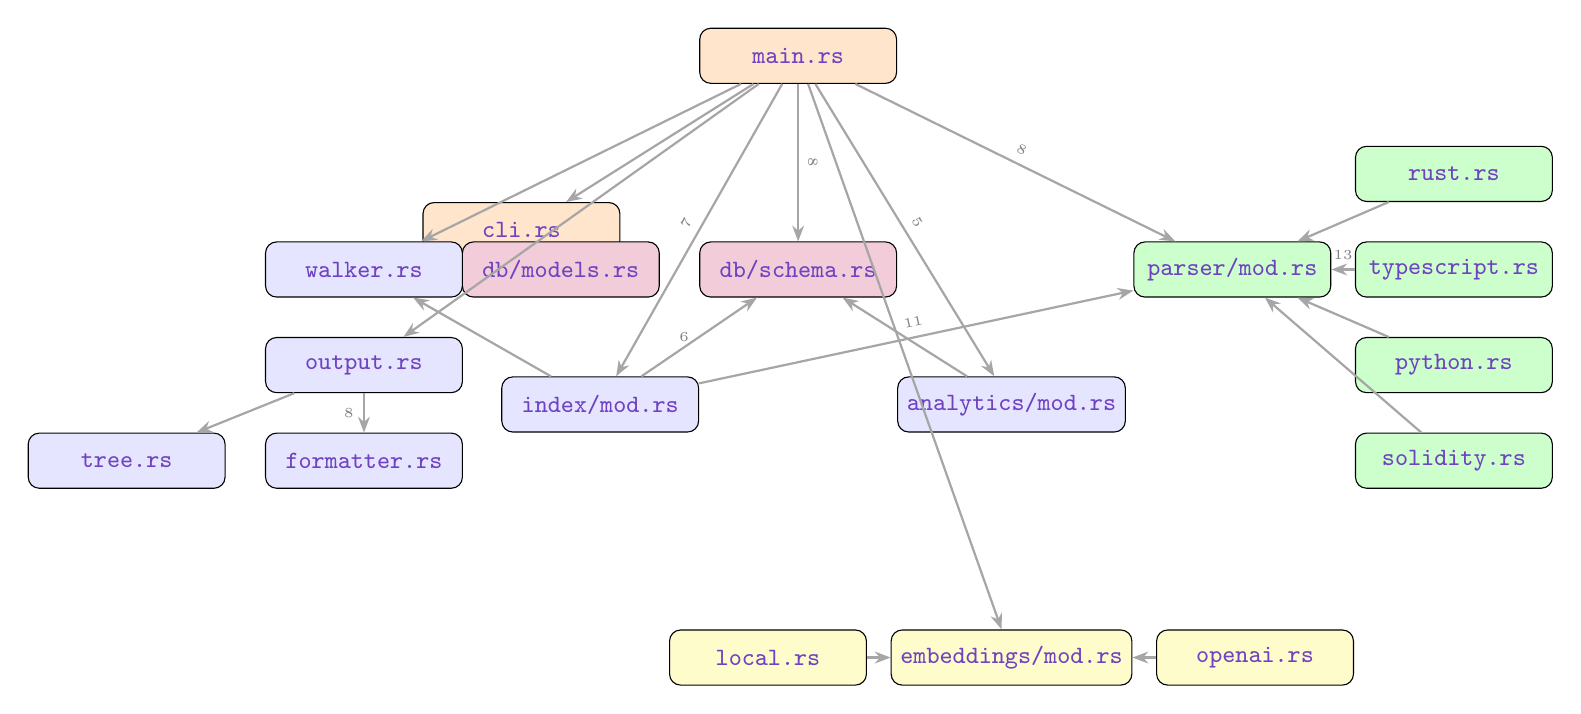
\begin{tikzpicture}[
    node distance=1.5cm,
    file/.style={rectangle, draw, rounded corners, minimum width=2.5cm, minimum height=0.7cm, align=center, fill=blue!10, font=\small},
    core/.style={file, fill=orange!20},
    parser/.style={file, fill=green!20},
    db/.style={file, fill=purple!20},
    arrow/.style={-{Stealth[length=2mm]}, thick, color=gray!70},
    label/.style={font=\tiny, color=gray}
]

% Core files
\node[core] (main) {\file{main.rs}};
\node[core, below left=1.5cm and 1cm of main] (cli) {\file{cli.rs}};

% Database layer
\node[db, below=2cm of main] (schema) {\file{db/schema.rs}};
\node[db, left=0.5cm of schema] (models) {\file{db/models.rs}};

% Parser layer
\node[parser, right=3cm of schema] (parsermod) {\file{parser/mod.rs}};
\node[parser, above right=0.5cm and 0.3cm of parsermod] (rust) {\file{rust.rs}};
\node[parser, right=0.3cm of parsermod] (ts) {\file{typescript.rs}};
\node[parser, below right=0.5cm and 0.3cm of parsermod] (py) {\file{python.rs}};
\node[parser, below=0.5cm of py] (sol) {\file{solidity.rs}};

% Index and analytics
\node[file, below left=1cm and 0cm of schema] (index) {\file{index/mod.rs}};
\node[file, below right=1cm and 0cm of schema] (analytics) {\file{analytics/mod.rs}};

% Context generation
\node[file, left=3cm of schema] (walker) {\file{walker.rs}};
\node[file, below=0.5cm of walker] (output) {\file{output.rs}};
\node[file, below=0.5cm of output] (formatter) {\file{formatter.rs}};
\node[file, left=0.5cm of formatter] (tree) {\file{tree.rs}};

% Embeddings
\node[file, fill=yellow!20, below=2.5cm of analytics] (embed) {\file{embeddings/mod.rs}};
\node[file, fill=yellow!20, left=0.3cm of embed] (local) {\file{local.rs}};
\node[file, fill=yellow!20, right=0.3cm of embed] (openai) {\file{openai.rs}};

% Arrows from main
\draw[arrow] (main) -- node[label, above, sloped] {8} (schema);
\draw[arrow] (main) -- node[label, above, sloped] {8} (parsermod);
\draw[arrow] (main) -- (cli);
\draw[arrow] (main) -- node[label, above, sloped] {7} (index);
\draw[arrow] (main) -- node[label, above, sloped] {5} (analytics);
\draw[arrow] (main) -- (walker);
\draw[arrow] (main) -- (output);
\draw[arrow] (main) -- (embed);

% Index dependencies
\draw[arrow] (index) -- node[label, above, sloped] {11} (parsermod);
\draw[arrow] (index) -- node[label, left] {6} (schema);
\draw[arrow] (index) -- (walker);

% Parser dependencies
\draw[arrow] (rust) -- (parsermod);
\draw[arrow] (ts) -- node[label, above] {13} (parsermod);
\draw[arrow] (py) -- (parsermod);
\draw[arrow] (sol) -- (parsermod);

% Output dependencies
\draw[arrow] (output) -- node[label, left] {8} (formatter);
\draw[arrow] (output) -- (tree);

% Analytics dependencies
\draw[arrow] (analytics) -- (schema);

% Embed dependencies
\draw[arrow] (local) -- (embed);
\draw[arrow] (openai) -- (embed);

\end{tikzpicture}
\caption{File-level dependency graph (numbers indicate call count)}
\label{fig:dependencies}
\end{figure}

\subsection{Key Dependency Chains}

\subsubsection{Main Entry Point}

The \file{main.rs} file serves as the central hub, with dependencies on most major modules:

\begin{verbatim}
main.rs ──┬──► db/schema.rs (8 calls)
          ├──► parser/mod.rs (8 calls)
          ├──► index/mod.rs (7 calls)
          ├──► analytics/mod.rs (5 calls)
          ├──► walker.rs
          ├──► output.rs
          ├──► formatter.rs
          └──► embeddings/mod.rs
\end{verbatim}

\subsubsection{Indexing Pipeline}

The indexing pipeline flows from file discovery through parsing to database storage:

\begin{verbatim}
index/mod.rs ──┬──► walker.rs (file discovery)
               ├──► parser/mod.rs (symbol extraction)
               │    └──► language-specific parsers
               └──► db/schema.rs (persistence)
\end{verbatim}

\subsubsection{Context Generation Pipeline}

Context generation is simpler, flowing from file selection through formatting:

\begin{verbatim}
output.rs ──┬──► walker.rs (file discovery)
            ├──► tree.rs (tree visualization)
            └──► formatter.rs (output formatting)
\end{verbatim}

\subsection{Parser Interdependencies}

An interesting pattern emerges in the parser modules---they have bidirectional dependencies:

\begin{verbatim}
typescript.rs ◄──► python.rs ◄──► rust.rs ◄──► solidity.rs
\end{verbatim}

This pattern likely arises from:
\begin{enumerate}
    \item Shared test fixtures imported across parsers
    \item Common type definitions used in all parsers
    \item Potential for further abstraction into a shared parser trait
\end{enumerate}

\subsection{Module Coupling Analysis}

\begin{table}[h]
\centering
\begin{tabular}{lrrr}
\toprule
\textbf{Module} & \textbf{Fan-Out} & \textbf{Fan-In} & \textbf{Coupling Score} \\
\midrule
\file{main.rs} & 43 & 0 & High (entry point) \\
\file{db/schema.rs} & 12 & 18 & High (central storage) \\
\file{parser/mod.rs} & 8 & 24 & High (shared utilities) \\
\file{index/mod.rs} & 18 & 8 & Medium \\
\file{formatter.rs} & 4 & 12 & Medium \\
\file{walker.rs} & 6 & 8 & Medium \\
\file{analytics/mod.rs} & 8 & 6 & Low \\
\file{embeddings/mod.rs} & 4 & 6 & Low \\
\bottomrule
\end{tabular}
\caption{Module coupling analysis}
\label{tab:coupling}
\end{table}

\subsection{Dependency Observations}

\subsubsection{Strengths}

\begin{itemize}
    \item \textbf{Clear layering} --- The codebase follows a clear layered architecture with minimal circular dependencies
    \item \textbf{Single responsibility} --- Each module has a focused purpose
    \item \textbf{Shared utilities} --- Common functionality is properly extracted to \file{parser/mod.rs}
    \item \textbf{Loose coupling for embeddings} --- The embedding system is well-isolated with a clean provider trait
\end{itemize}

\subsubsection{Areas for Improvement}

\begin{itemize}
    \item \textbf{main.rs coupling} --- The main file has high coupling to many modules; consider extracting command handlers to separate modules
    \item \textbf{Parser interdependencies} --- The bidirectional dependencies between parsers could be reduced by extracting shared test utilities
    \item \textbf{db/schema.rs size} --- With 74 symbols, this module handles many responsibilities; consider splitting into smaller focused modules
\end{itemize}

\subsection{Recommended Refactoring}

\subsubsection{Extract Command Handlers}

Move command-specific logic from \file{main.rs} to dedicated modules:

\begin{verbatim}
src/
├── commands/
│   ├── mod.rs
│   ├── index.rs      # Index command handler
│   ├── query.rs      # Query command handlers
│   ├── search.rs     # Search command handler
│   ├── embed.rs      # Embedding command handler
│   └── context.rs    # Context generation handler
├── main.rs           # Entry point only
└── ...
\end{verbatim}

\subsubsection{Split Database Module}

Separate concerns within the database layer:

\begin{verbatim}
src/db/
├── mod.rs            # Re-exports
├── schema.rs         # Schema definitions
├── symbols.rs        # Symbol CRUD operations
├── edges.rs          # Edge CRUD operations
├── search.rs         # FTS5 search operations
├── embeddings.rs     # Embedding storage
└── migrations.rs     # Schema migrations
\end{verbatim}

\subsubsection{Create Parser Trait}

Unify parser implementations behind a common trait:

\begin{lstlisting}[style=rustcode, caption={Proposed parser trait}]
pub trait LanguageParser {
    fn language(&self) -> Language;
    fn symbols_query(&self) -> &str;
    fn calls_query(&self) -> &str;
    
    fn extract_symbols(&self, tree: &Tree, source: &str) -> Vec<Symbol>;
    fn extract_edges(&self, tree: &Tree, source: &str) -> Vec<Edge>;
}

// Then in mod.rs:
pub fn get_parser(language: Language) -> Box<dyn LanguageParser> {
    match language {
        Language::Rust => Box::new(RustParser::new()),
        Language::TypeScript => Box::new(TypeScriptParser::new()),
        // ...
    }
}
\end{lstlisting}

% ============================================================================
% STRENGTHS
% ============================================================================

\section{Codebase Strengths}
\label{sec:strengths}

This section highlights the positive aspects of the \ctx{} codebase that demonstrate good software engineering practices.

\subsection{Clean Module Separation}

The codebase exhibits excellent separation of concerns:

\begin{itemize}
    \item \textbf{Context Generation} is isolated from \textbf{Code Intelligence}
    \item Each language parser is self-contained in its own file
    \item Database operations are separated from business logic
    \item Embedding providers are abstracted behind a common trait
\end{itemize}

This separation enables:
\begin{itemize}
    \item Independent testing of each module
    \item Easy addition of new features without affecting existing code
    \item Clear boundaries for code review and ownership
\end{itemize}

\subsection{Trait-Based Extensibility}

The codebase makes excellent use of Rust traits for extensibility:

\subsubsection{Formatter Trait}

\begin{lstlisting}[style=rustcode]
pub trait Formatter {
    fn start(&self, tree_block: Option<&str>) -> String;
    fn format_file(&self, path: &str, content: &str) -> String;
    fn end(&self) -> String;
}
\end{lstlisting}

This allows easy addition of new output formats (JSON, YAML, etc.) without modifying existing code.

\subsubsection{EmbeddingProvider Trait}

\begin{lstlisting}[style=rustcode]
pub trait EmbeddingProvider {
    fn embed(&self, texts: &[String]) -> Result<Vec<Vec<f32>>>;
    fn dimension(&self) -> usize;
}
\end{lstlisting}

Enables support for multiple embedding backends (local, OpenAI, future providers) with a unified interface.

\subsection{Incremental Processing}

The indexing system implements intelligent incremental updates:

\begin{itemize}
    \item \textbf{Content hashing} instead of timestamps for reliable change detection
    \item \textbf{Selective re-parsing} only for modified files
    \item \textbf{Batch updates} for efficiency during full reindex
    \item \textbf{Watch mode} for real-time index updates during development
\end{itemize}

\begin{lstlisting}[style=rustcode, caption={Content hash-based change detection}]
fn needs_update(&self, path: &str, content: &str) -> bool {
    let new_hash = sha256(content);
    match self.db.get_hash(path) {
        Some(old_hash) => new_hash != old_hash,
        None => true, // New file
    }
}
\end{lstlisting}

\subsection{Dual Storage Strategy}

The combination of SQLite and DuckDB provides the best of both worlds:

\begin{table}[h]
\centering
\begin{tabular}{lll}
\toprule
\textbf{Aspect} & \textbf{SQLite} & \textbf{DuckDB} \\
\midrule
Purpose & Persistent storage & Analytical queries \\
Optimization & OLTP (transactions) & OLAP (analytics) \\
Storage & Single file on disk & In-memory \\
Queries & Simple CRUD & Recursive CTEs \\
\bottomrule
\end{tabular}
\caption{Dual storage strategy comparison}
\label{tab:storage-comparison}
\end{table}

Benefits:
\begin{itemize}
    \item No data duplication---DuckDB reads directly from SQLite
    \item Single source of truth for all data
    \item Optimal performance for each query type
    \item Simple deployment with no additional infrastructure
\end{itemize}

\subsection{Comprehensive Language Support}

Six languages are supported with deep parsing capabilities:

\begin{itemize}
    \item \textbf{Rust} --- Functions, structs, enums, traits, impl blocks, doc comments
    \item \textbf{TypeScript/JavaScript} --- Functions, classes, interfaces, types, JSDoc
    \item \textbf{Python} --- Functions, classes, decorators, async functions, docstrings
    \item \textbf{Solidity} --- Contracts, functions, events, errors, NatSpec comments
\end{itemize}

Each parser extracts:
\begin{itemize}
    \item Symbol definitions with signatures
    \item Call relationships between functions
    \item Import/export relationships
    \item Inheritance and implementation edges
    \item Documentation strings
\end{itemize}

\subsection{Streaming Output Support}

For large codebases, the context generation system supports streaming:

\begin{lstlisting}[style=rustcode, caption={Streaming context generation}]
pub fn stream_context<W: Write>(
    writer: &mut W,
    files: &[PathBuf],
    formatter: &dyn Formatter,
) -> io::Result<()> {
    // Stream header
    write!(writer, "{}", formatter.stream_start(tree_block))?;
    
    // Stream each file individually
    for file in files {
        let content = fs::read_to_string(file)?;
        write!(writer, "{}", formatter.stream_file(path, &content))?;
    }
    
    // Stream footer
    write!(writer, "{}", formatter.stream_end())?;
    Ok(())
}
\end{lstlisting}

Benefits:
\begin{itemize}
    \item Memory-efficient for large codebases
    \item Immediate output feedback
    \item Pipeline-friendly for shell composition
\end{itemize}

\subsection{Robust Ignore System}

A three-tier ignore system ensures clean context generation:

\begin{enumerate}
    \item \textbf{.gitignore} --- Standard git ignore patterns (default enabled)
    \item \textbf{.contextignore} --- Project-specific exclusions for LLM context
    \item \textbf{Built-in patterns} --- 170+ patterns for common non-source files
\end{enumerate}

Categories of built-in ignores:
\begin{itemize}
    \item Version control directories (\code{.git/}, \code{.svn/})
    \item Dependencies (\code{node\_modules/}, \code{vendor/}, \code{target/})
    \item Build outputs (\code{dist/}, \code{build/}, \code{.next/})
    \item Binary files (images, executables, archives)
    \item Lock files (\code{package-lock.json}, \code{Cargo.lock})
    \item Secrets (\code{.env}, \code{*.pem}, \code{*.key})
\end{itemize}

\subsection{Good Test Coverage}

The codebase includes comprehensive tests:

\begin{itemize}
    \item \textbf{Unit tests} for parser symbol extraction
    \item \textbf{Unit tests} for call edge detection
    \item \textbf{Integration tests} for indexing workflows
    \item \textbf{Snapshot tests} for output formatting
\end{itemize}

Example test pattern:

\begin{lstlisting}[style=rustcode, caption={Parser test example}]
#[test]
fn test_extract_rust_symbols() {
    let source = r#"
        pub fn hello() {}
        struct User { name: String }
        impl User {
            pub fn new() -> Self { User { name: String::new() } }
        }
    "#;
    
    let symbols = extract_symbols(source, Language::Rust);
    
    assert!(symbols.iter().any(|s| s.name == "hello"));
    assert!(symbols.iter().any(|s| s.name == "User"));
    assert!(symbols.iter().any(|s| s.name == "new"));
}
\end{lstlisting}

\subsection{Documentation Quality}

The project includes comprehensive documentation:

\begin{itemize}
    \item \textbf{README.md} --- Quick start and feature overview
    \item \textbf{docs/} directory with detailed guides:
    \begin{itemize}
        \item Getting started guide
        \item Architecture documentation
        \item Code intelligence reference
        \item Configuration guide
        \item Language support details
    \end{itemize}
    \item \textbf{Inline documentation} --- Doc comments on public APIs
    \item \textbf{Examples} --- Command-line examples throughout docs
\end{itemize}

% ============================================================================
% AREAS FOR IMPROVEMENT
% ============================================================================

\section{Areas for Improvement}
\label{sec:improvements}

This section identifies opportunities for improving the \ctx{} codebase based on the analysis findings.

\subsection{High Complexity Functions}

\subsubsection{Problem}

The \func{extract\_symbols} functions in each parser handle too many responsibilities, leading to high fan-out counts (42--48 calls each).

\subsubsection{Current State}

\begin{lstlisting}[style=rustcode, caption={Current monolithic extract\_symbols (simplified)}]
pub fn extract_symbols(tree: &Tree, source: &str) -> Vec<Symbol> {
    let mut symbols = Vec::new();
    let query = Query::new(language(), SYMBOLS_QUERY)?;
    let mut cursor = QueryCursor::new();
    
    for match_ in cursor.matches(&query, tree.root_node(), source.as_bytes()) {
        // Symbol metadata extraction
        let name = get_capture_text(&match_, "name", source);
        let kind = determine_kind(&match_);
        
        // Signature building (complex logic)
        let signature = build_signature(&match_, source);
        
        // Docstring extraction
        let docstring = extract_docstring(&match_, source);
        
        // Visibility determination
        let visibility = determine_visibility(&match_);
        
        // Parent tracking
        let parent_id = find_parent(&match_, &symbols);
        
        symbols.push(Symbol { name, kind, signature, docstring, visibility, parent_id });
    }
    symbols
}
\end{lstlisting}

\subsubsection{Recommended Refactoring}

Decompose into smaller, focused functions:

\begin{lstlisting}[style=rustcode, caption={Proposed decomposition}]
pub fn extract_symbols(tree: &Tree, source: &str) -> Vec<Symbol> {
    let matches = run_symbols_query(tree, source);
    
    matches.into_iter()
        .map(|m| build_symbol_from_match(m, source))
        .collect()
}

fn run_symbols_query(tree: &Tree, source: &str) -> Vec<QueryMatch> {
    let query = Query::new(language(), SYMBOLS_QUERY)?;
    QueryCursor::new()
        .matches(&query, tree.root_node(), source.as_bytes())
        .collect()
}

fn build_symbol_from_match(match_: QueryMatch, source: &str) -> Symbol {
    Symbol {
        name: extract_name(&match_, source),
        kind: determine_kind(&match_),
        signature: build_signature(&match_, source),
        brief: extract_docstring(&match_, source),
        visibility: determine_visibility(&match_),
        parent_id: None, // Resolve in post-processing
    }
}
\end{lstlisting}

\subsection{Duplicate Formatter Code}

\subsubsection{Problem}

The \code{Formatter} trait implementations share significant code, particularly in \func{stream\_start} and \func{wrap} methods (85--88\% similarity).

\subsubsection{Recommended Solution}

Use default trait methods:

\begin{lstlisting}[style=rustcode, caption={Formatter with default implementations}]
pub trait Formatter {
    // Required methods
    fn name(&self) -> &'static str;
    fn content_wrapper(&self) -> (&'static str, &'static str);
    fn file_header(&self, path: &str) -> String;
    fn file_footer(&self) -> String;
    
    // Default implementations
    fn start(&self, tree_block: Option<&str>) -> String {
        let (start, _) = self.content_wrapper();
        match tree_block {
            Some(tree) => format!("{}\n{}\n", start, tree),
            None => start.to_string(),
        }
    }
    
    fn end(&self) -> String {
        let (_, end) = self.content_wrapper();
        end.to_string()
    }
    
    fn format_file(&self, path: &str, content: &str) -> String {
        format!("{}{}{}", 
            self.file_header(path),
            content,
            self.file_footer()
        )
    }
}
\end{lstlisting}

\subsection{Error Handling Consistency}

\subsubsection{Problem}

Error handling is inconsistent across modules:
\begin{itemize}
    \item Some functions use \code{io::Error}
    \item Others use \code{Box<dyn Error>}
    \item Embeddings use custom \code{EmbeddingError}
    \item Database uses \code{rusqlite::Error}
\end{itemize}

\subsubsection{Recommended Solution}

Create a unified error type using \code{thiserror}:

\begin{lstlisting}[style=rustcode, caption={Unified error type}]
use thiserror::Error;

#[derive(Error, Debug)]
pub enum CtxError {
    #[error("IO error: {0}")]
    Io(#[from] std::io::Error),
    
    #[error("Database error: {0}")]
    Database(#[from] rusqlite::Error),
    
    #[error("Parser error: {0}")]
    Parser(String),
    
    #[error("Embedding error: {0}")]
    Embedding(#[from] EmbeddingError),
    
    #[error("Query error: {0}")]
    Query(String),
    
    #[error("Configuration error: {0}")]
    Config(String),
}

pub type Result<T> = std::result::Result<T, CtxError>;
\end{lstlisting}

\subsection{Parser Abstraction}

\subsubsection{Problem}

Each parser implements similar patterns independently, leading to:
\begin{itemize}
    \item Code duplication
    \item Inconsistent behavior
    \item Difficulty adding new languages
\end{itemize}

\subsubsection{Recommended Solution}

Create a \code{LanguageParser} trait:

\begin{lstlisting}[style=rustcode, caption={LanguageParser trait}]
pub trait LanguageParser: Send + Sync {
    /// The tree-sitter language for this parser
    fn ts_language(&self) -> tree_sitter::Language;
    
    /// Query for extracting symbols
    fn symbols_query(&self) -> &str;
    
    /// Query for extracting call edges
    fn calls_query(&self) -> &str;
    
    /// Map capture names to symbol kinds
    fn kind_mapping(&self) -> &[(& str, SymbolKind)];
    
    /// Extract symbols from parsed tree (can override for custom logic)
    fn extract_symbols(&self, tree: &Tree, source: &str) -> Vec<Symbol> {
        // Default implementation using symbols_query()
        default_extract_symbols(self, tree, source)
    }
    
    /// Extract edges from parsed tree (can override for custom logic)
    fn extract_edges(&self, tree: &Tree, source: &str) -> Vec<Edge> {
        // Default implementation using calls_query()
        default_extract_edges(self, tree, source)
    }
}

// Factory function
pub fn parser_for(language: Language) -> Option<Box<dyn LanguageParser>> {
    match language {
        Language::Rust => Some(Box::new(RustParser)),
        Language::TypeScript => Some(Box::new(TypeScriptParser)),
        Language::Python => Some(Box::new(PythonParser)),
        Language::Solidity => Some(Box::new(SolidityParser)),
        _ => None,
    }
}
\end{lstlisting}

\subsection{Configuration Management}

\subsubsection{Problem}

Configuration is scattered across:
\begin{itemize}
    \item Command-line arguments
    \item Hardcoded values in source
    \item Environment variables (only \code{OPENAI\_API\_KEY})
\end{itemize}

\subsubsection{Recommended Solution}

Implement a configuration file system:

\begin{lstlisting}[style=bashcode, caption={Example .ctx/config.toml}]
# .ctx/config.toml

[index]
watch_debounce_ms = 500
batch_size = 50
exclude_patterns = ["*.generated.*", "vendor/"]

[embeddings]
provider = "local"  # or "openai"
dimension = 384
batch_size = 100

[output]
default_format = "xml"
show_sizes = false
include_tree = true

[complexity]
threshold = 10
warn_on_high = true
\end{lstlisting}

Configuration loading:

\begin{lstlisting}[style=rustcode, caption={Configuration loading}]
#[derive(Deserialize, Default)]
pub struct Config {
    #[serde(default)]
    pub index: IndexConfig,
    #[serde(default)]
    pub embeddings: EmbeddingsConfig,
    #[serde(default)]
    pub output: OutputConfig,
}

impl Config {
    pub fn load() -> Result<Self> {
        let config_path = Path::new(".ctx/config.toml");
        if config_path.exists() {
            let content = fs::read_to_string(config_path)?;
            Ok(toml::from_str(&content)?)
        } else {
            Ok(Config::default())
        }
    }
}
\end{lstlisting}

\subsection{Missing JSON Formatter}

\subsubsection{Problem}

The \func{get\_formatter} function has an incomplete JSON format implementation:

\begin{lstlisting}[style=rustcode]
OutputFormat::Json => Box::new(PlainFormatter), // TODO: Implement JSON formatter
\end{lstlisting}

\subsubsection{Recommended Implementation}

\begin{lstlisting}[style=rustcode, caption={JSON formatter implementation}]
pub struct JsonFormatter;

impl Formatter for JsonFormatter {
    fn start(&self, tree_block: Option<&str>) -> String {
        let tree = tree_block.map(|t| json!(t)).unwrap_or(json!(null));
        format!(r#"{{"project_tree": {}, "files": ["#, tree)
    }
    
    fn format_file(&self, path: &str, content: &str) -> String {
        let file = json!({
            "path": path,
            "content": content
        });
        file.to_string()
    }
    
    fn end(&self) -> String {
        "]}".to_string()
    }
}
\end{lstlisting}

\subsection{Summary of Recommendations}

\begin{table}[h]
\centering
\begin{tabular}{llc}
\toprule
\textbf{Issue} & \textbf{Solution} & \textbf{Priority} \\
\midrule
High complexity functions & Decompose into smaller functions & High \\
Duplicate formatter code & Default trait methods & Medium \\
Inconsistent error handling & Unified \code{CtxError} type & Medium \\
Parser code duplication & \code{LanguageParser} trait & Medium \\
Scattered configuration & Config file support & Low \\
Missing JSON formatter & Implement \code{JsonFormatter} & Low \\
\bottomrule
\end{tabular}
\caption{Improvement recommendations summary}
\label{tab:recommendations}
\end{table}

% ============================================================================
% STATISTICS
% ============================================================================

\section{Codebase Statistics}
\label{sec:statistics}

This section presents detailed statistics about the \ctx{} codebase.

\subsection{Overall Metrics}

\begin{table}[h]
\centering
\begin{tabular}{lr}
\toprule
\textbf{Metric} & \textbf{Value} \\
\midrule
Total Source Files & 20 \\
Total Lines of Code & $\approx$ 8,500 \\
Total Symbols & 548 \\
Total Edges (Relationships) & 2,664 \\
\bottomrule
\end{tabular}
\caption{Overall codebase metrics}
\label{tab:overall-metrics}
\end{table}

\subsection{Symbol Distribution}

\begin{table}[h]
\centering
\begin{tabular}{lrr}
\toprule
\textbf{Symbol Kind} & \textbf{Count} & \textbf{Percentage} \\
\midrule
Functions & 446 & 81.4\% \\
Structs & 35 & 6.4\% \\
Enums & 11 & 2.0\% \\
Traits & 3 & 0.5\% \\
Constants & 53 & 9.7\% \\
\midrule
\textbf{Total} & \textbf{548} & \textbf{100\%} \\
\bottomrule
\end{tabular}
\caption{Symbol distribution by kind}
\label{tab:symbol-distribution}
\end{table}

\subsection{Per-File Breakdown}

\begin{longtable}{lrrrr}
\toprule
\textbf{File} & \textbf{Total} & \textbf{Functions} & \textbf{Public} & \textbf{Types} \\
\midrule
\endhead
\file{main.rs} & 43 & 38 & 2 & 0 \\
\file{db/schema.rs} & 74 & 65 & 52 & 3 \\
\file{parser/mod.rs} & 40 & 32 & 28 & 4 \\
\file{formatter.rs} & 47 & 42 & 38 & 3 \\
\file{parser/typescript.rs} & 41 & 36 & 8 & 2 \\
\file{parser/python.rs} & 44 & 40 & 8 & 1 \\
\file{index/mod.rs} & 34 & 28 & 15 & 2 \\
\file{analytics/mod.rs} & 31 & 26 & 18 & 2 \\
\file{embeddings/mod.rs} & 29 & 24 & 18 & 3 \\
\file{parser/rust.rs} & 26 & 22 & 6 & 1 \\
\file{embeddings/openai.rs} & 25 & 22 & 4 & 1 \\
\file{parser/solidity.rs} & 22 & 19 & 5 & 1 \\
\file{embeddings/local.rs} & 21 & 18 & 4 & 1 \\
\file{db/models.rs} & 28 & 12 & 12 & 9 \\
\file{cli.rs} & 18 & 8 & 8 & 6 \\
\file{tree.rs} & 15 & 12 & 8 & 1 \\
\file{walker.rs} & 14 & 11 & 8 & 1 \\
\file{output.rs} & 10 & 8 & 6 & 1 \\
\file{default\_ignores.rs} & 3 & 2 & 2 & 0 \\
\bottomrule
\caption{Symbol count per file}
\label{tab:per-file}
\end{longtable}

\subsection{Edge Distribution}

\begin{table}[h]
\centering
\begin{tabular}{lrr}
\toprule
\textbf{Edge Kind} & \textbf{Count} & \textbf{Percentage} \\
\midrule
Calls & 2,412 & 90.5\% \\
Imports & 198 & 7.4\% \\
Extends & 32 & 1.2\% \\
Implements & 22 & 0.8\% \\
\midrule
\textbf{Total} & \textbf{2,664} & \textbf{100\%} \\
\bottomrule
\end{tabular}
\caption{Edge distribution by kind}
\label{tab:edge-distribution}
\end{table}

\subsection{Most Connected Functions}

Functions with the highest connectivity (combined fan-in and fan-out):

\begin{table}[h]
\centering
\begin{tabular}{lrrr}
\toprule
\textbf{Function} & \textbf{Fan-Out} & \textbf{Fan-In} & \textbf{Total} \\
\midrule
\func{extract\_symbols} (typescript) & 48 & 4 & 52 \\
\func{extract\_symbols} (solidity) & 48 & 4 & 52 \\
\func{discover\_files} & 46 & 2 & 48 \\
\func{parse\_response} & 45 & 1 & 46 \\
\func{parse} (typescript) & 20 & 43 & 63 \\
\func{extract\_symbols} (rust) & 42 & 3 & 45 \\
\func{watch\_and\_index} & 41 & 1 & 42 \\
\func{build\_signature} (typescript) & 39 & 2 & 41 \\
\func{extract\_call\_edges} & 37 & 4 & 41 \\
\func{run\_query} & 37 & 1 & 38 \\
\bottomrule
\end{tabular}
\caption{Most connected functions}
\label{tab:connected-functions}
\end{table}

\subsection{Code Quality Metrics}

\begin{table}[h]
\centering
\begin{tabular}{lr}
\toprule
\textbf{Quality Metric} & \textbf{Value} \\
\midrule
Functions analyzed & 446 \\
High complexity functions & 17 (3.8\%) \\
Critical complexity functions & 0 (0\%) \\
Duplicate code pairs (80\%+ similarity) & 13 \\
Average function fan-out & 6.0 \\
Median function fan-out & 4 \\
Maximum function fan-out & 48 \\
Functions with zero fan-out & 89 (20\%) \\
\bottomrule
\end{tabular}
\caption{Code quality metrics}
\label{tab:quality-metrics}
\end{table}

\subsection{Language Distribution}

All source files are written in Rust:

\begin{table}[h]
\centering
\begin{tabular}{lrr}
\toprule
\textbf{Language} & \textbf{Files} & \textbf{Percentage} \\
\midrule
Rust & 20 & 100\% \\
\bottomrule
\end{tabular}
\caption{Source file language distribution}
\label{tab:language-dist}
\end{table}

\subsection{Module Size Distribution}

\begin{figure}[h]
\centering
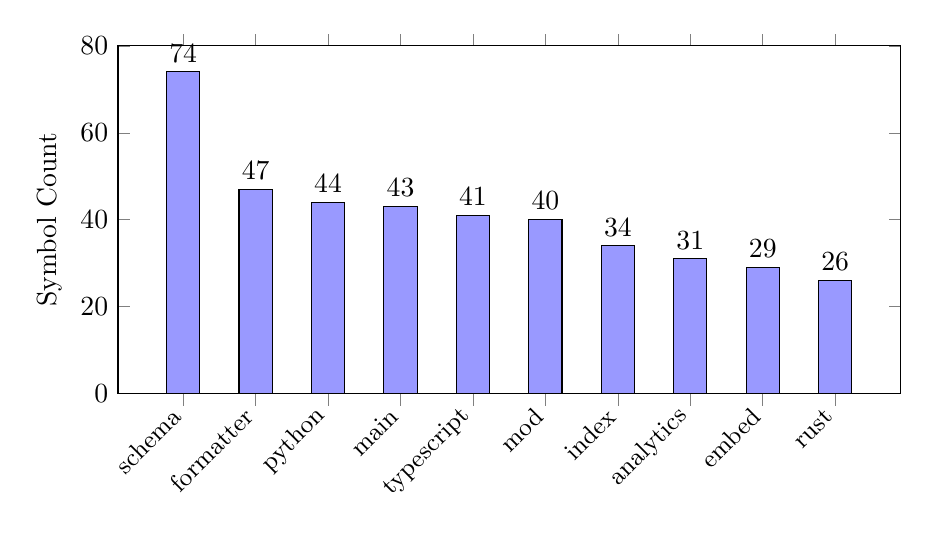
\begin{tikzpicture}
\begin{axis}[
    ybar,
    ylabel={Symbol Count},
    symbolic x coords={schema, formatter, python, main, typescript, mod, index, analytics, embed, rust},
    xtick=data,
    x tick label style={rotate=45, anchor=east, font=\small},
    ymin=0,
    ymax=80,
    bar width=12pt,
    nodes near coords,
    nodes near coords align={vertical},
    width=0.95\textwidth,
    height=6cm,
]
\addplot[fill=blue!40] coordinates {
    (schema, 74)
    (formatter, 47)
    (python, 44)
    (main, 43)
    (typescript, 41)
    (mod, 40)
    (index, 34)
    (analytics, 31)
    (embed, 29)
    (rust, 26)
};
\end{axis}
\end{tikzpicture}
\caption{Top 10 modules by symbol count}
\label{fig:module-size}
\end{figure}

\subsection{Test Coverage Areas}

The codebase includes tests for the following areas:

\begin{itemize}
    \item \textbf{Parser tests} --- Symbol extraction and call edge detection for each language
    \item \textbf{Formatter tests} --- Output format correctness
    \item \textbf{Database tests} --- CRUD operations and query correctness
    \item \textbf{Walker tests} --- File discovery and ignore patterns
    \item \textbf{Integration tests} --- End-to-end indexing workflows
\end{itemize}

\subsection{External Dependencies}

Key external crates used:

\begin{table}[h]
\centering
\begin{tabular}{ll}
\toprule
\textbf{Crate} & \textbf{Purpose} \\
\midrule
\code{clap} & Command-line argument parsing \\
\code{rusqlite} & SQLite database access \\
\code{duckdb} & Analytical queries \\
\code{tree-sitter} & Source code parsing \\
\code{tree-sitter-*} & Language-specific grammars \\
\code{ignore} & Gitignore-style file filtering \\
\code{fastembed} & Local embedding generation \\
\code{reqwest} & HTTP client for OpenAI API \\
\code{serde} & Serialization/deserialization \\
\code{flate2} & Gzip compression \\
\code{sha2} & Content hashing \\
\code{notify} & File system watching \\
\bottomrule
\end{tabular}
\caption{Key external dependencies}
\label{tab:dependencies}
\end{table}

% ============================================================================
% CONCLUSION
% ============================================================================

\section{Conclusion}
\label{sec:conclusion}

\subsection{Summary}

The \ctx{} codebase is a well-structured Rust CLI tool that successfully provides two valuable capabilities:

\begin{enumerate}
    \item \textbf{Context Generation} --- Efficiently formats source code for LLM consumption with multiple output formats, intelligent filtering, and streaming support.
    
    \item \textbf{Code Intelligence} --- Comprehensive code analysis including indexing, full-text search, semantic search with embeddings, call graph generation, and impact analysis.
\end{enumerate}

The analysis reveals a codebase with:
\begin{itemize}
    \item \textbf{548 symbols} across \textbf{20 source files}
    \item \textbf{2,664 edges} representing function calls and relationships
    \item \textbf{Clear module separation} between concerns
    \item \textbf{Extensible design} through traits and provider patterns
    \item \textbf{Efficient storage} using SQLite for persistence and DuckDB for analytics
\end{itemize}

\subsection{Key Strengths}

\begin{enumerate}
    \item \textbf{Architecture} --- Clean separation between context generation and code intelligence, with well-defined module boundaries.
    
    \item \textbf{Extensibility} --- Trait-based design for formatters and embedding providers enables easy extension.
    
    \item \textbf{Performance} --- Incremental indexing, content hashing, and streaming output provide excellent performance characteristics.
    
    \item \textbf{Language Support} --- Comprehensive parsing for six languages with consistent symbol and edge extraction.
    
    \item \textbf{Storage Strategy} --- Innovative dual-database approach combines SQLite persistence with DuckDB analytics.
\end{enumerate}

\subsection{Areas for Improvement}

\begin{enumerate}
    \item \textbf{Complexity Reduction} --- The 17 high-complexity functions, particularly the \func{extract\_symbols} functions in parsers, should be decomposed into smaller, focused functions.
    
    \item \textbf{Code Deduplication} --- The 13 identified duplicate code pairs should be addressed through default trait implementations and shared utilities.
    
    \item \textbf{Error Handling} --- Implement a unified error type across all modules for consistent error handling.
    
    \item \textbf{Parser Abstraction} --- Create a \code{LanguageParser} trait to reduce duplication and simplify adding new languages.
    
    \item \textbf{Configuration} --- Add support for a configuration file to centralize settings currently scattered across CLI arguments and hardcoded values.
\end{enumerate}

\subsection{Recommended Next Steps}

Based on this analysis, we recommend the following prioritized actions:

\begin{table}[h]
\centering
\begin{tabular}{clp{8cm}}
\toprule
\textbf{Priority} & \textbf{Action} & \textbf{Rationale} \\
\midrule
1 & Refactor \func{extract\_symbols} & Highest complexity, affects all parsers \\
2 & Implement \code{LanguageParser} trait & Reduces duplication, simplifies maintenance \\
3 & Add default \code{Formatter} methods & Eliminates duplicate formatter code \\
4 & Create unified \code{CtxError} type & Improves error handling consistency \\
5 & Implement JSON formatter & Completes output format support \\
6 & Add configuration file support & Improves user experience \\
\bottomrule
\end{tabular}
\caption{Recommended action priority}
\label{tab:action-priority}
\end{table}

\subsection{Final Assessment}

The \ctx{} codebase demonstrates solid software engineering practices and is well-positioned for future development. The identified improvements are refinements rather than fundamental issues---the core architecture is sound and the tool provides genuine value for developers working with LLMs.

The combination of context generation and code intelligence in a single, fast CLI tool fills an important gap in the developer tooling ecosystem. With the recommended improvements, \ctx{} could become an even more robust and maintainable tool.

\begin{center}
\rule{0.5\textwidth}{0.4pt}
\end{center}

\begin{flushright}
\textit{Analysis generated using \ctx{} code intelligence features}\\
\textit{\today}
\end{flushright}


\end{document}
